\documentclass[12pt]{article}
\usepackage[margin=1in]{geometry}
\usepackage{graphicx}
\usepackage{booktabs}
\usepackage{amsmath}
\title{The Effect of Paid Search Advertising on Revenue: \\
A Replication of the eBay Natural Experiment}
\author{andrewmoon}
\date{\today}
\begin{document}
\maketitle
\section{Introduction}

Firms spend billions of dollars each year on search engine marketing (SEM), 
yet measuring its causal effect on sales is difficult. When a consumer searches 
for a product online, it is often unclear whether a paid advertisement actually 
drives the purchase or whether the consumer would have found the company through 
organic search results anyway. This makes it challenging for firms to determine 
the true return on investment of paid search advertising.

This paper examines the effect of paid search advertising on eBay's revenue 
using a natural experiment studied by Blake, Nosko, and Tadelis (2014). 
In this experiment, eBay temporarily stopped bidding on search advertisements 
in a subset of geographic markets while continuing advertising in others. 
By comparing changes in revenue between these groups before and after the change, 
we can estimate the causal impact of paid search using a difference-in-differences (DID) approach.
\section{Experimental Setting}

The analysis is based on a large-scale field experiment conducted by eBay and studied 
by Blake, Nosko, and Tadelis (2014). Beginning on May 22, 2012, eBay stopped bidding 
on Google AdWords advertisements in 65 designated market areas (DMAs) in the United States. 
These markets form the treatment group. In the remaining 145 DMAs, eBay continued 
its paid search advertising as usual, forming the control group. The experiment lasted 
for approximately eight weeks.

Importantly, the experiment was not fully randomized. The largest DMAs were excluded 
from treatment because eBay expected that turning off advertising in these markets 
could significantly affect revenue. As a result, the treatment and control groups 
differ in their baseline levels of revenue, with control markets generally having 
higher average sales. Because of this baseline difference, a simple comparison of 
average revenue across groups would not provide a valid estimate of the treatment 
effect. Instead, this paper uses a difference-in-differences approach that compares 
how revenue changes over time within each group.
\section{Data and Figures}

The dataset contains daily revenue observations for 210 designated market areas 
between April and July 2012. Each observation records the date, the DMA identifier, 
whether the market belongs to the treatment or control group, and the revenue generated 
by eBay in that market on that day. The treatment period begins on May 22, 2012, 
when paid search advertising was turned off in the treatment DMAs.

Figure \ref{fig:revenue} shows the average daily revenue for the treatment and control 
groups over time. The dashed vertical line marks the start of the treatment period.
\begin{figure}[h]
\centering
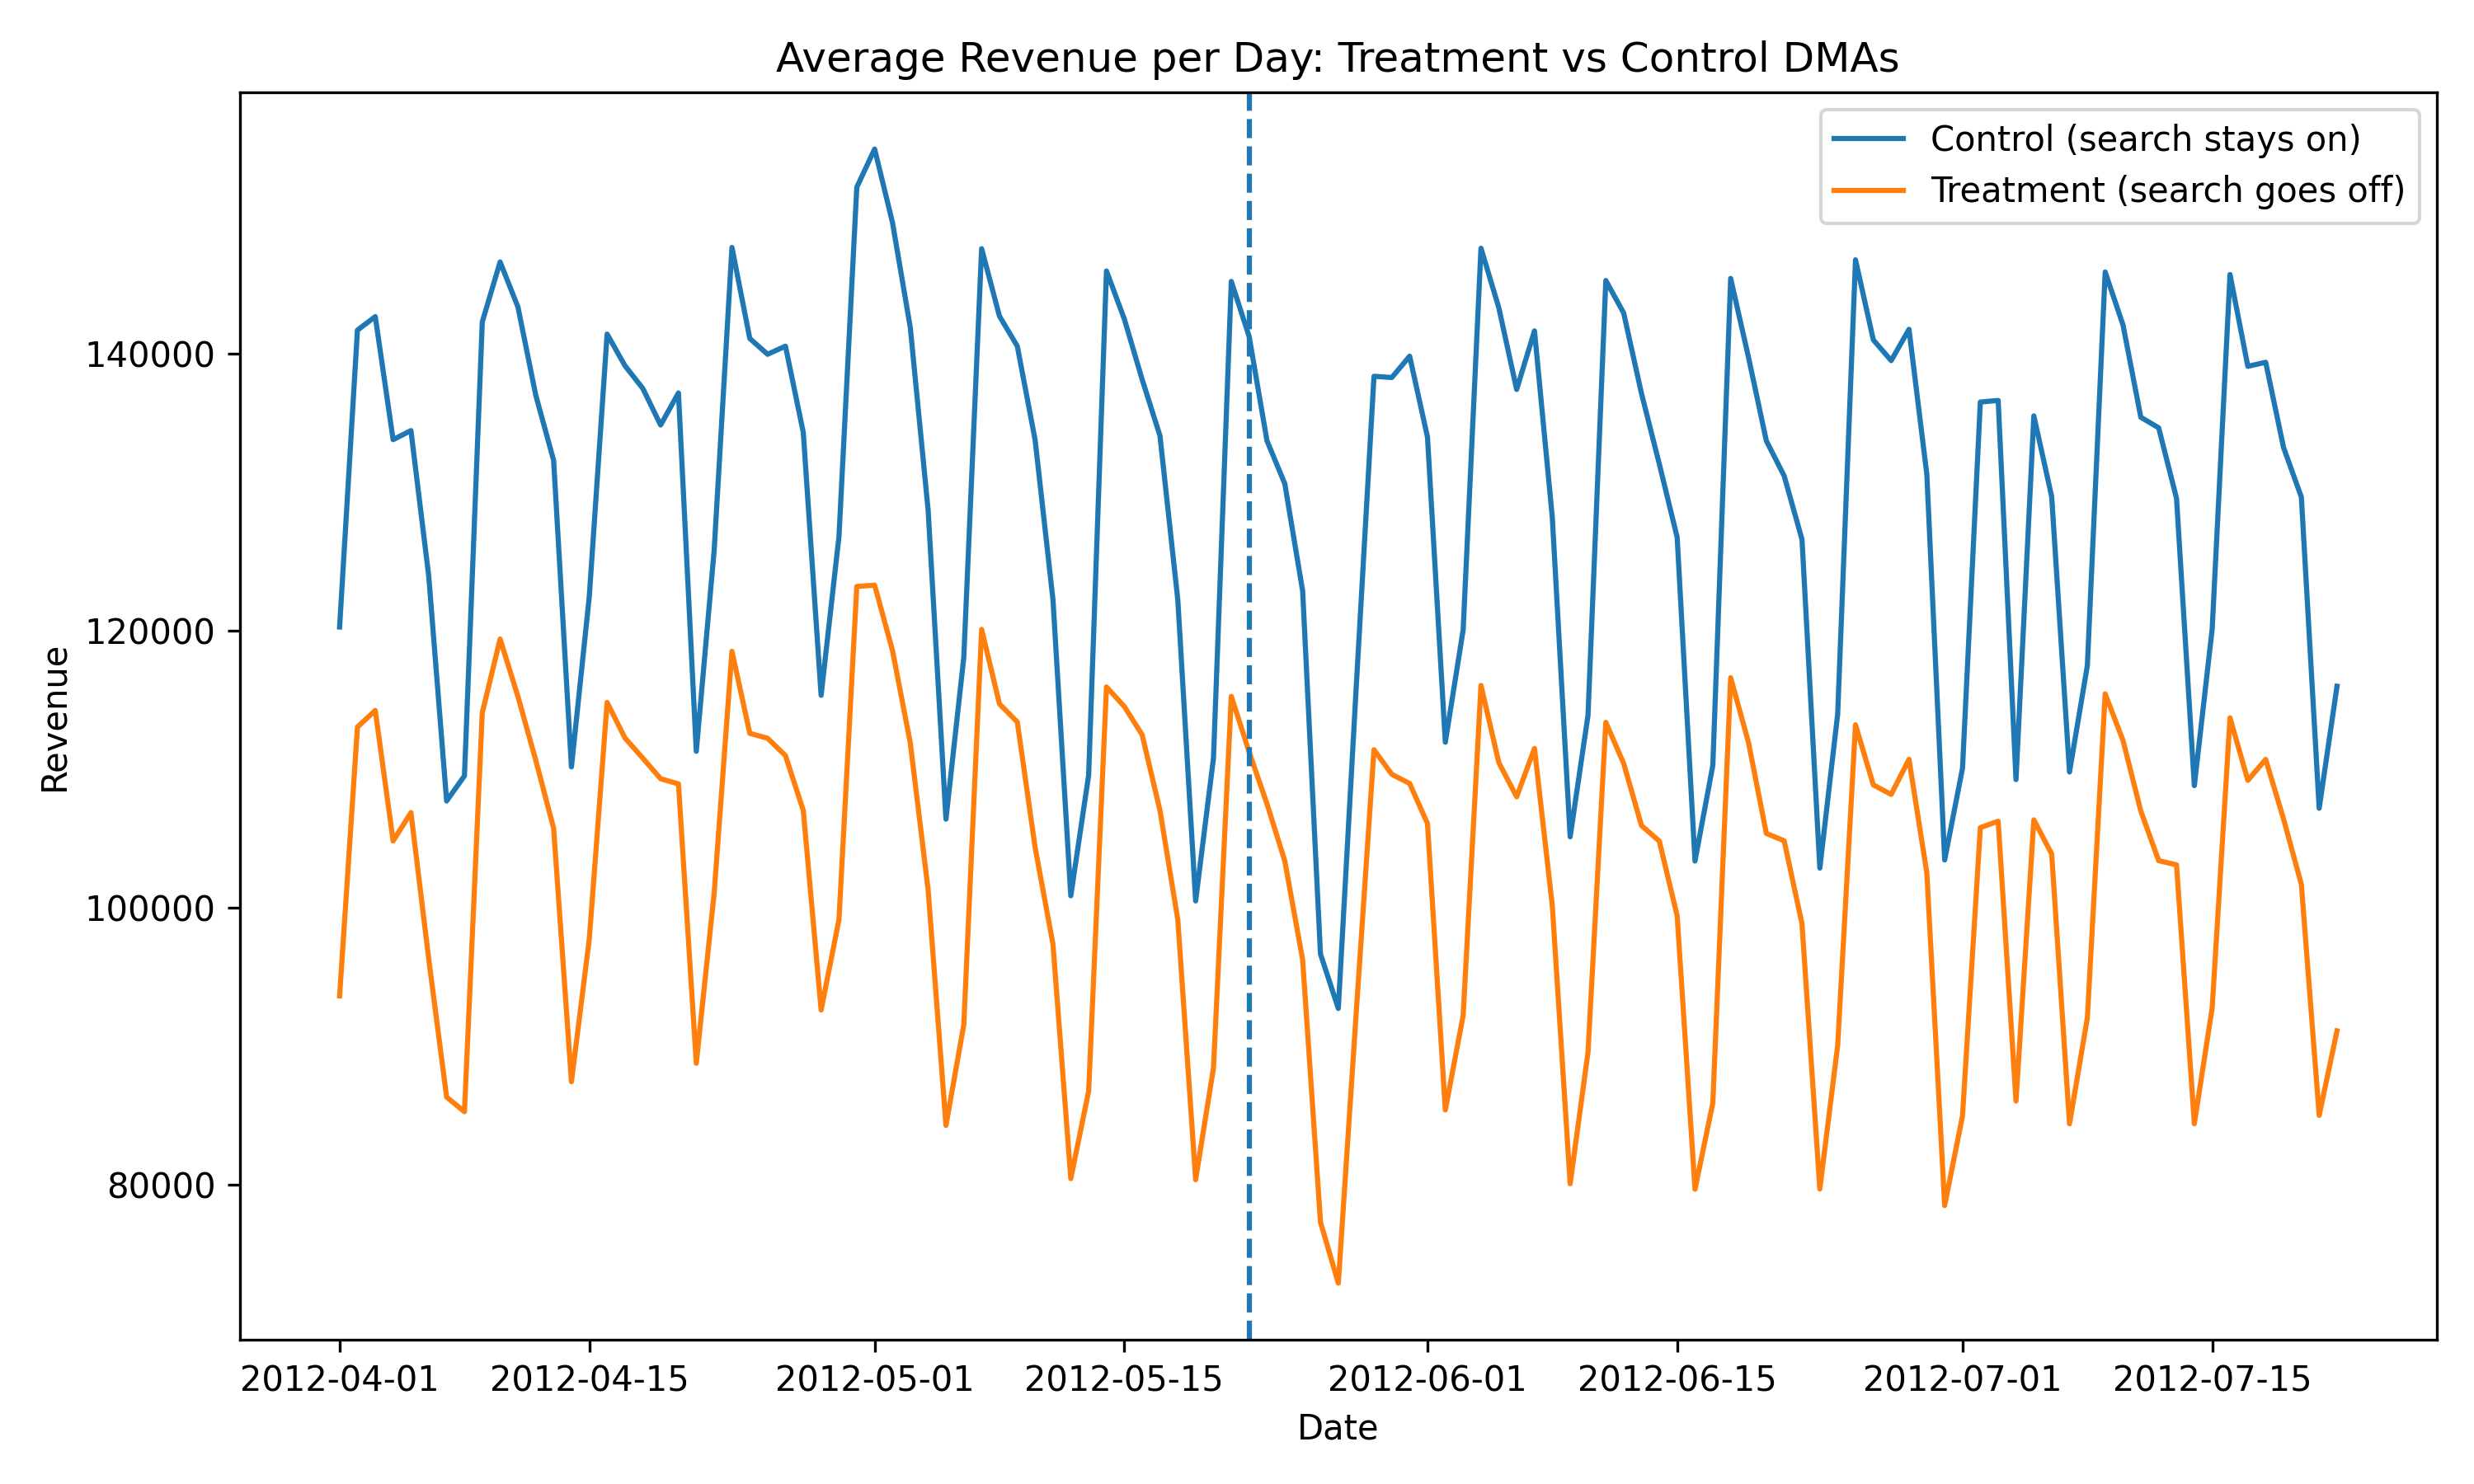
\includegraphics[width=0.85\textwidth]{../output/figures/figure_5_2.png}
\caption{Average revenue for treatment and control DMAs over time.
The dashed line marks May 22, 2012, when SEM was turned off
for the treatment group.}
\label{fig:revenue}
\end{figure}

The figure shows that the control group consistently has higher average revenue 
than the treatment group. This difference reflects the experimental design, 
since the largest markets were excluded from the treatment group. Both groups 
display similar weekly oscillation patterns, suggesting that they follow similar 
seasonal demand patterns. At this scale, it is difficult to visually identify a clear 
divergence in revenue trends after the treatment begins.

\begin{figure}[h]
\centering
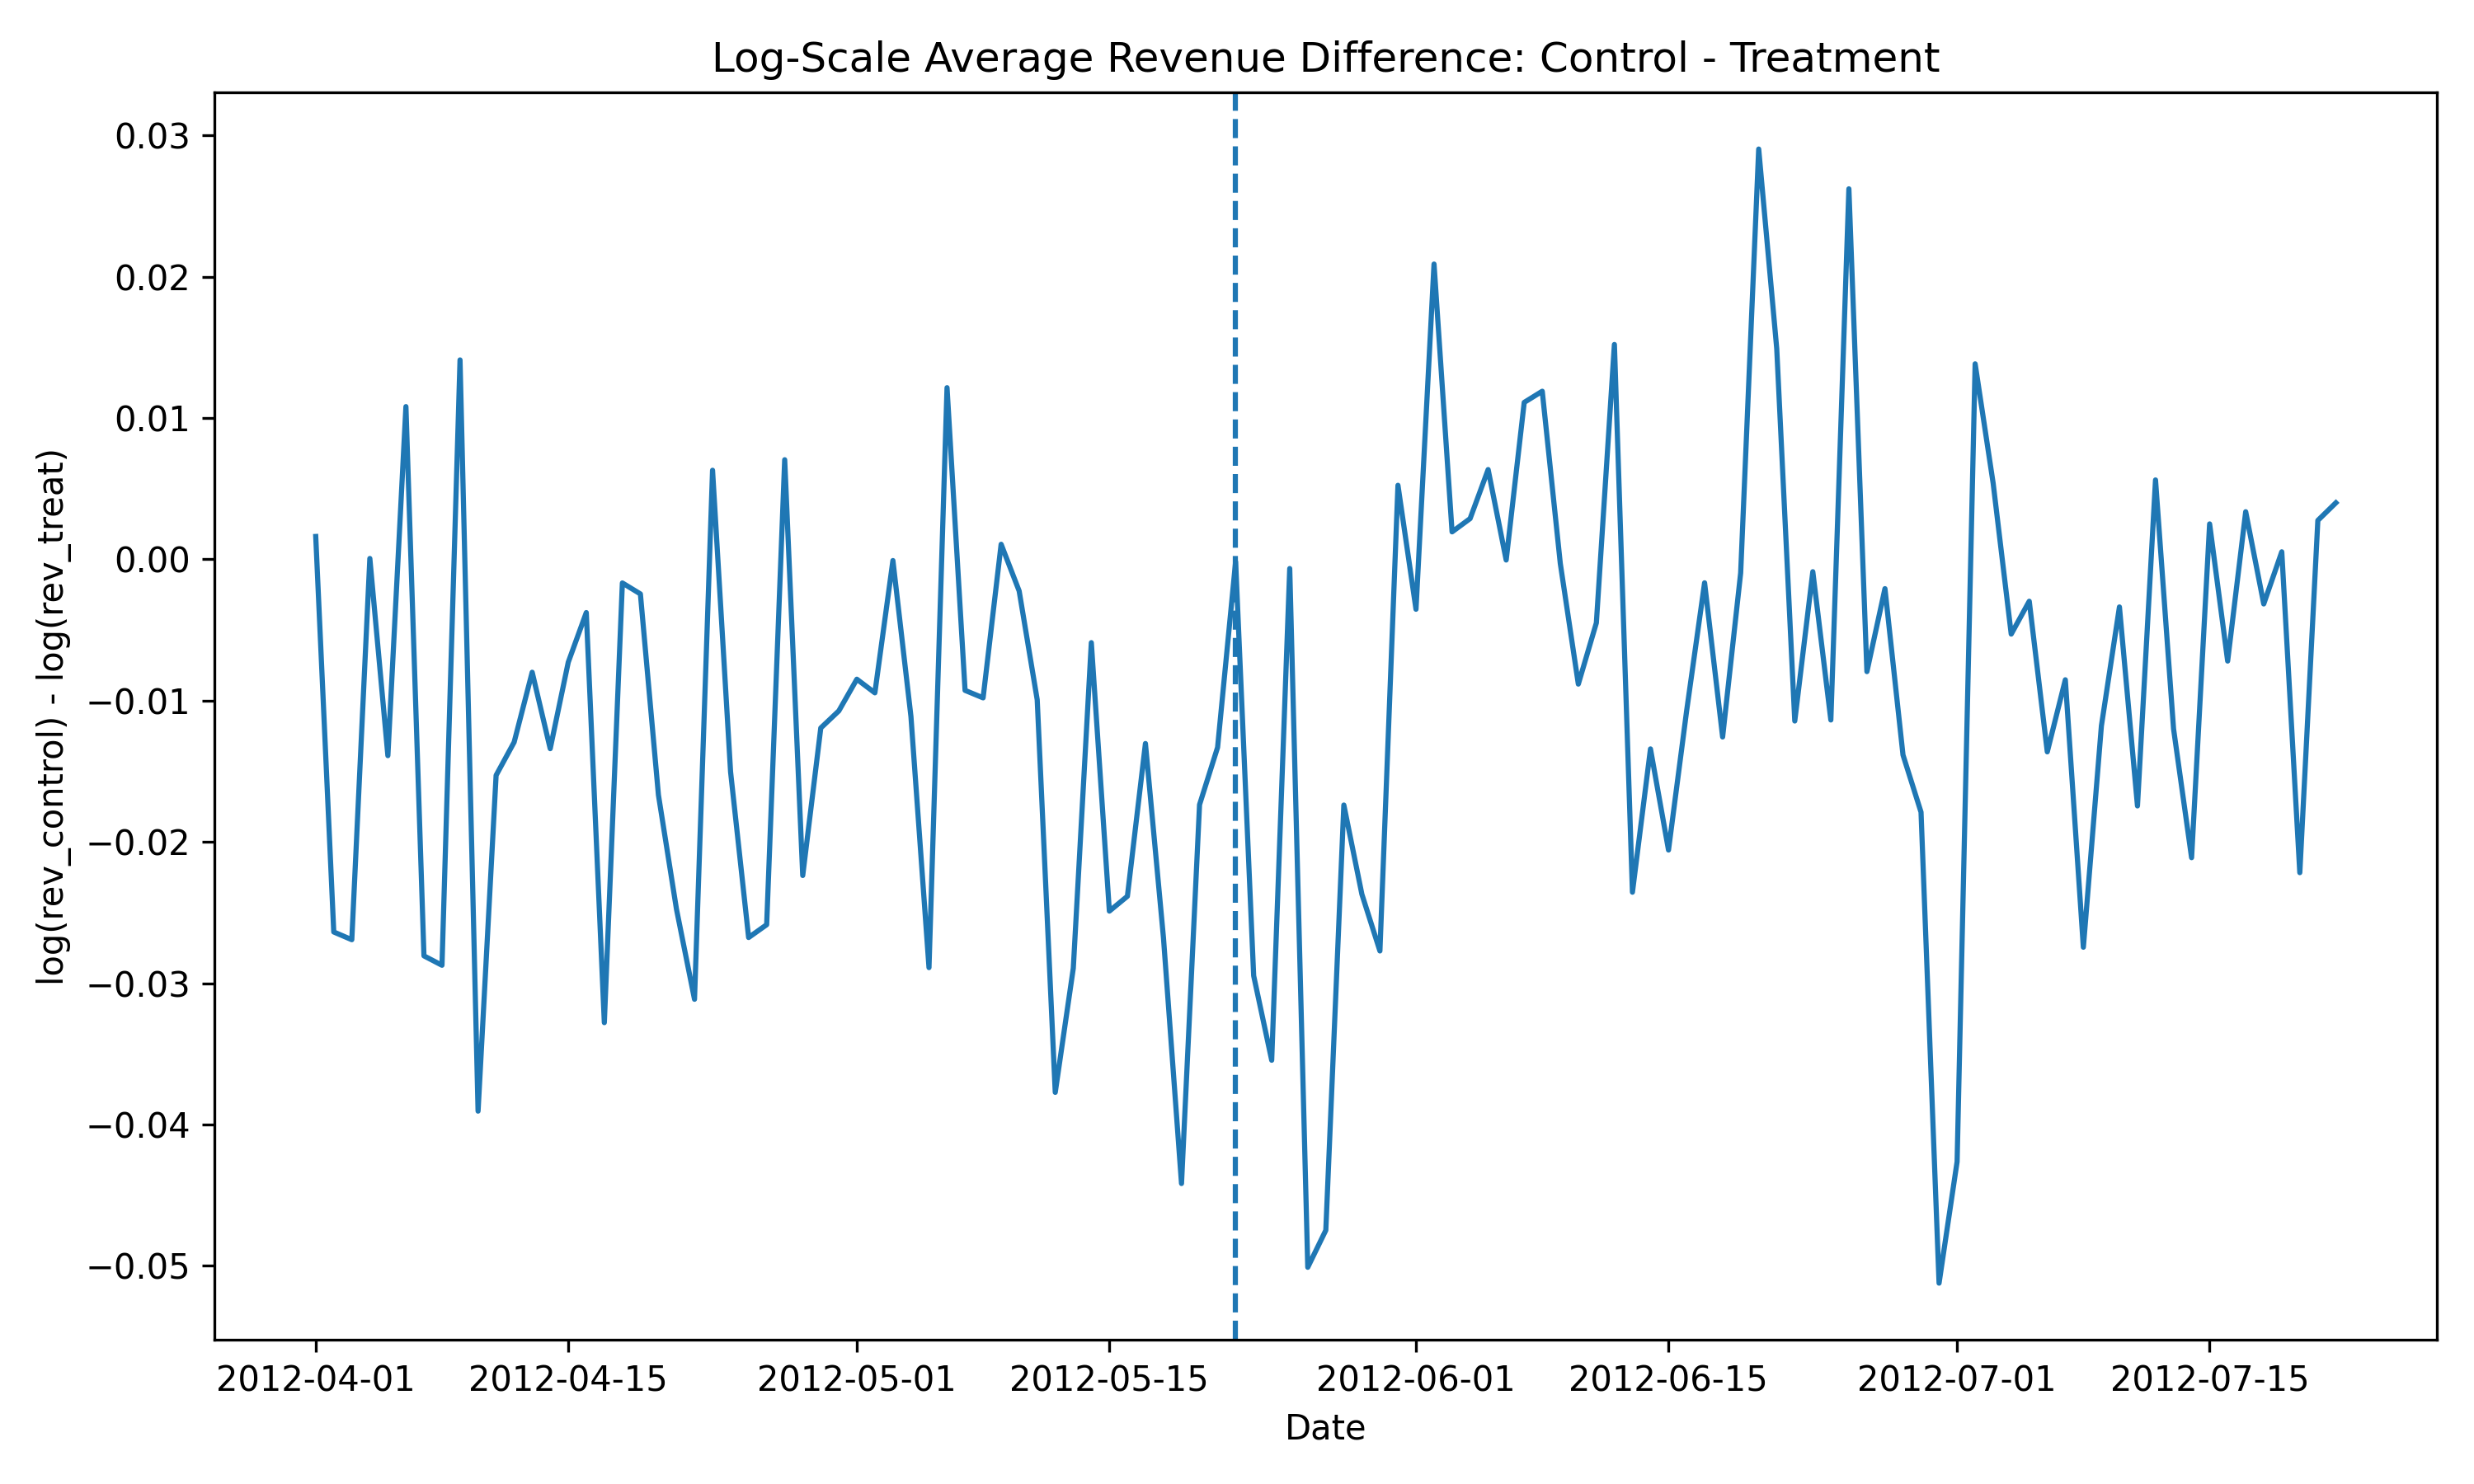
\includegraphics[width=0.85\textwidth]{../output/figures/figure_5_3.png}
\caption{Log-scale average revenue difference between control and treatment
groups over time. The gap appears to increase after May 22.}
\label{fig:logdiff}
\end{figure}

Figure \ref{fig:logdiff} plots the difference in log average revenue between the 
control and treatment groups over time. Before May 22, the gap fluctuates around 
a relatively stable level, indicating that the two groups follow similar trends 
prior to the intervention. After the treatment begins, the gap appears to increase 
slightly, suggesting that revenue in the treatment markets may have fallen relative 
to the control markets. This visual pattern motivates the formal difference-in-differences 
analysis presented in the next section.

\section{Results}
% Include the DID table
\input{../output/tables/did_table.tex}

Table \ref{tab:did} reports the difference-in-differences estimate of the effect of 
turning off paid search advertising on revenue. The estimated treatment effect is 
$\hat{\gamma} = -0.0066$ in log scale. Converting this estimate to levels implies that 
revenue in the treatment markets declined by approximately $0.66\%$ after paid 
search advertising was turned off.

However, the estimated effect is not statistically significant at conventional 
levels. The 95\% confidence interval ranges from $-0.0175$ to $0.0043$, which includes 
zero. This means we cannot reject the hypothesis that paid search advertising had 
no measurable effect on revenue during the experiment period.

Economically, this result suggests that paid search advertising contributes little 
incremental revenue for a well-known brand such as eBay. Many users who search for 
eBay may already intend to visit the website and would find it through organic search 
results even in the absence of paid advertisements.

\section{Conclusion}

This paper replicates a difference-in-differences analysis of eBay's paid search 
advertising experiment. The results suggest that turning off paid search advertising 
reduced revenue by approximately 0.66 percent, but the effect is not statistically 
significant. These findings replicate the main conclusion of Blake, Nosko, and 
Tadelis (2014), which is that paid search advertising has a very small effect on 
revenue for a well-known brand.

Several limitations should be noted. The dataset used in this replication is 
scaled and does not represent actual revenue values, and the experiment was not 
fully randomized across markets. In addition, the analysis uses a simple 
difference-in-differences estimator rather than a more detailed regression 
framework with additional controls. Despite these limitations, the results highlight 
the importance of using experimental or quasi-experimental methods when 
evaluating the effectiveness of marketing strategies.

\begin{thebibliography}{9}
\bibitem{blake2014}
Blake, T., C. Nosko, and S. Tadelis (2014).
``Consumer Heterogeneity and Paid Search Effectiveness: A Large-Scale Field Experiment.''
\textit{Econometrica}, 83(1): 155--174.
\bibitem{taddy2019}
Taddy, M. (2019).

\textit{Business Data Science}. McGraw-Hill, Chapter 5.
\end{thebibliography}
\end{document}
